\section{Text-to-Speech (TTS) \& Vocoders}

\begin{frame}{}
    \LARGE \textbf{Text-to-Speech (TTS) \& Vocoders}
\end{frame}

\begin{frame}[allowframebreaks]{Speech Synthesis (Text-to-Speech)}

\begin{itemize}
    \item Speech synthesis, also known as Text-to-Speech (TTS), converts written text into spoken audio.

    \item How it works:
    \begin{itemize}
        \item \textbf{Input:} raw text.
        \item \textbf{Processing:} linguistic analysis → acoustic modeling → vocoder.
        \item \textbf{Output:} waveform (audio file).
    \end{itemize}

    \item Why it matters:
    \begin{itemize}
        \item Accessibility: screen readers for visually impaired users.
        \item Voice assistants, audiobooks, GPS navigation, and language learning applications.
    \end{itemize}

    \item Example:
    \begin{itemize}
        \item Text: ``Welcome to the lecture'' → synthetic speech audio output.
    \end{itemize}
\end{itemize}
\framebreak
    \begin{itemize}
        \item Applications: virtual assistants, accessibility, entertainment
        \item Key components:
        \begin{itemize}
            \item Text analysis
            \item Acoustic modeling
            \item Vocoder synthesis
        \end{itemize}
    \end{itemize}
    \begin{center}
        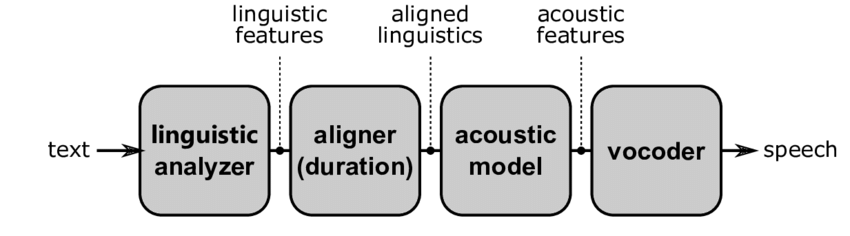
\includegraphics[width=0.8\textwidth,height=0.9\textheight,keepaspectratio]{images/audio-nlp/tts_pipeline.png}
    \end{center}
\end{frame}

\begin{frame}[allowframebreaks]{Traditional TTS Pipeline}

\begin{itemize}
    \item Traditional TTS uses a modular pipeline where each stage handles a specific aspect of text-to-speech conversion.

    \item Pipeline steps:
    \begin{enumerate}
        \item \textbf{Text Analysis:} normalize numbers, abbreviations, and punctuation.
        \item \textbf{Phonetic Analysis:} convert graphemes to phonemes.
        \item \textbf{Prosody Modeling:} predict rhythm, intonation, and stress patterns.
        \item \textbf{Acoustic Model:} generate spectrogram-like features representing speech.
        \item \textbf{Vocoder:} convert acoustic features into a waveform (audio output).
    \end{enumerate}

    \item Advantages and limitations:
    \begin{itemize}
        \item Clear, interpretable stages.
        \item Hand-engineered, less flexible than modern neural TTS approaches.
    \end{itemize}
\end{itemize}

\end{frame}

\begin{frame}[allowframebreaks]{Statistical Parametric TTS}

\begin{itemize}
    \item Statistical Parametric TTS generates speech by modeling acoustic and prosody parameters statistically, often using Hidden Markov Models (HMMs).

    \item How it works:
    \begin{itemize}
        \item Acoustic and prosody features are predicted via HMMs.
        \item Vocoder converts predicted features into a speech waveform.
    \end{itemize}

    \item Advantages:
    \begin{itemize}
        \item Smaller model footprint.
        \item Flexible, can adapt to new speakers or styles with limited data.
    \end{itemize}

    \item Limitations:
    \begin{itemize}
        \item Synthesized speech often sounds muffled or buzzy compared to natural human speech.
    \end{itemize}
\end{itemize}

\begin{figure}
        \centering
        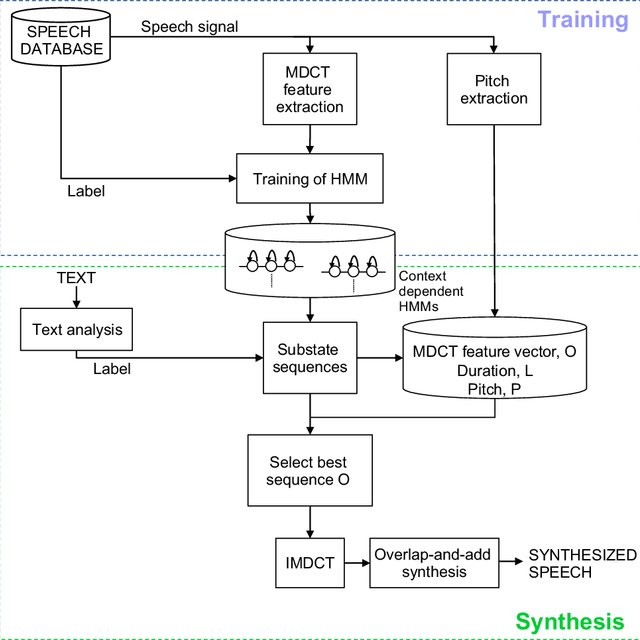
\includegraphics[width=\textwidth,height=0.8\textheight,keepaspectratio]{images/audio-nlp-eval/tts-hmm-based.png}
        \caption*{HMM-based TTS diagram. Source: \href{https://www.researchgate.net/figure/The-scheme-of-an-HMM-based-TTS-system_fig1_328565312}{ResearchGate}}
    \end{figure}

\end{frame}


\begin{frame}[allowframebreaks]{Tacotron 2}
    \begin{itemize}
        \item End-to-end TTS system
        \item Pipeline:
        \begin{itemize}
            \item Text $\rightarrow$ Mel-spectrogram (sequence-to-sequence model)
            \item Mel-spectrogram $\rightarrow$ WaveNet/GAN vocoder (audio synthesis)
        \end{itemize}
        \item Improved prosody and pronunciation
        \item Flexible for different voices and languages
    \end{itemize}
    \begin{center}
        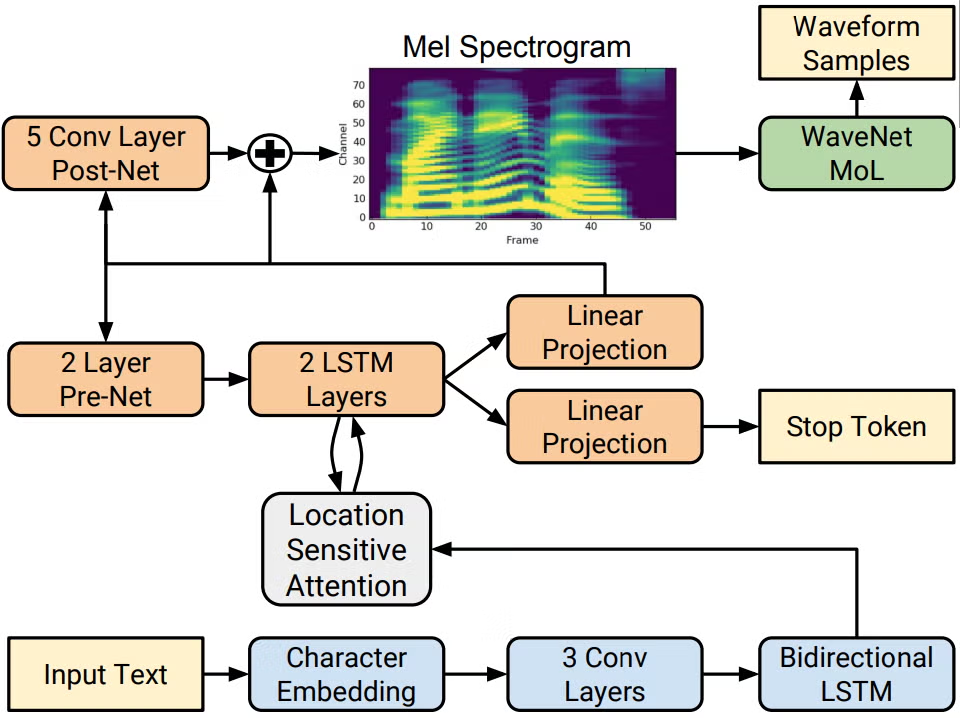
\includegraphics[width=\textwidth,height=0.9\textheight,keepaspectratio]{images/audio-nlp/tacotron2_pipeline.png}
    \end{center}
\end{frame}

\begin{frame}[allowframebreaks]{FastSpeech, HiFi-GAN, Glow-TTS, Diffusion Models}
    \begin{itemize}
        \setlength{\itemsep}{1.5em}
        \item Non-autoregressive models: faster inference
        \item FastSpeech:
        \begin{itemize}
            \item Parallel generation of spectrograms
            \item Duration prediction for alignment
        \end{itemize}
        \item HiFi-GAN:
        \begin{itemize}
            \item GAN-based vocoder
            \item High-fidelity, real-time synthesis
        \end{itemize}
    \framebreak
        \item Glow-TTS:
        \begin{itemize}
            \item Flow-based generative model
            \item Efficient and expressive speech synthesis
        \end{itemize}
        \item Diffusion models:
        \begin{itemize}
            \item Iterative refinement of audio
            \item State-of-the-art naturalness
        \end{itemize}
    \end{itemize}
    \begin{center}
        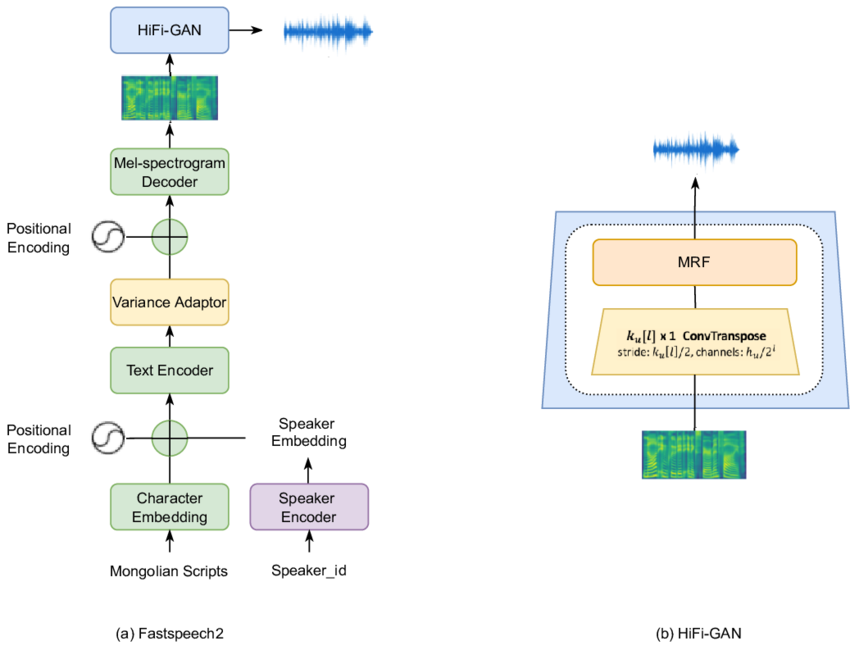
\includegraphics[width=\textwidth,height=0.9\textheight,keepaspectratio]{images/audio-nlp/fastspeech_hifigan.png}
    \end{center}
\end{frame}


\begin{frame}[allowframebreaks]{Neural Vocoders}

\begin{itemize}
    \item Neural vocoders convert intermediate representations (e.g., spectrograms) into waveforms, producing high-quality speech.

    \item Popular approaches:
    \begin{itemize}
        \item \textbf{WaveNet (2016):} autoregressive model, produces very natural speech but relatively slow.
        \item \textbf{WaveGlow, Parallel WaveGAN, HiFi-GAN:} faster, real-time neural vocoders.
    \end{itemize}

    \item Core idea (WaveNet):
    \[
        p(\mathbf{x}) = \prod_t p(x_t \mid x_{<t})
    \]
    Each audio sample is modeled conditionally on all previous samples.

    \item Why it matters:
    \begin{itemize}
        \item The quality of the vocoder directly impacts the perceived naturalness of synthesized speech.
    \end{itemize}
\end{itemize}
\begin{figure}
        \centering
        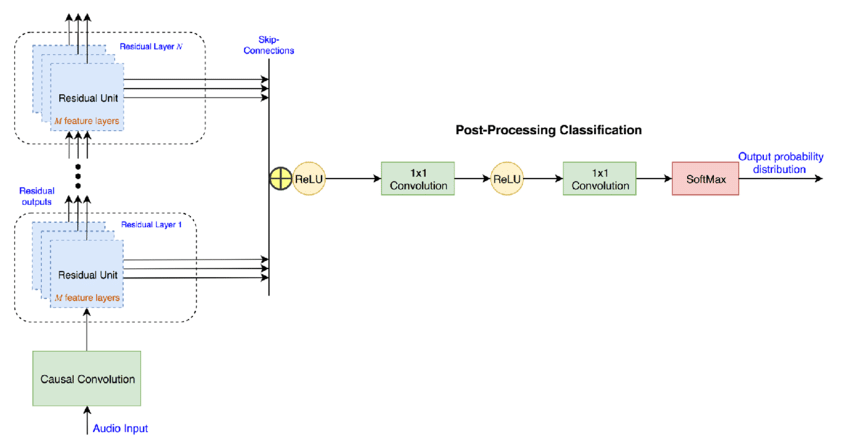
\includegraphics[width=\textwidth,height=0.8\textheight,keepaspectratio]{images/audio-nlp/wavenet_architecture.png}
        \caption*{WaveNet architecture. Source: \href{https://deepmind.com/blog/article/wavenet-generative-model-raw-audio}{DeepMind}}
    \end{figure}

\end{frame}


\begin{frame}[allowframebreaks]{Evaluating TTS}

\begin{itemize}
    \item Measuring TTS quality requires both human judgment and objective metrics.

    \item Common evaluation methods:
    \begin{itemize}
        \item \textbf{MOS (Mean Opinion Score):} human listeners rate naturalness on a 1–5 scale.
        \item \textbf{AB preference tests:} humans choose their preferred sample between two systems.
        \item \textbf{Objective metrics:} 
        \begin{itemize}
            \item MCD (Mel-Cepstral Distortion)  
            \item PESQ (Perceptual Evaluation of Speech Quality)
        \end{itemize}
    \end{itemize}

    \item Why evaluation matters:
    \begin{itemize}
        \item Human perception is the ultimate measure of speech quality.
        \item Automated metrics help accelerate development and iteration.
    \end{itemize}
\end{itemize}

\end{frame}


\begin{frame}[allowframebreaks]{Challenges in TTS}

\begin{itemize}
    \item Modern TTS systems face several practical and ethical challenges:

    \item \textbf{Prosody & Emotion:}  
    Generating natural intonation, emphasis, and expressive speech remains difficult.

    \item \textbf{Cross-Speaker Synthesis:}  
    Voice cloning or multi-speaker synthesis requires adapting models to new voices without losing quality.

    \item \textbf{Low-Resource Languages:}  
    Limited data makes it challenging to build high-quality TTS systems for many languages.

    \item \textbf{Ethical Issues:}  
    Risk of misuse in deepfakes or generating fake celebrity voices.
\end{itemize}

\end{frame}
